\documentclass[../main.tex]{subfiles}

\begin{document}

\subsection{Simulation and reinforcement learning}

\lipsum[1]

\subsection{Object detection}

\lipsum[1]

\subsection{Physical components}
The most critical parts in the hardware
architecture are the Raspberry Pi and the drone. 
So we started by configuring the Raspberry Pi sd-card,
flashed it with Ubuntu 18.04 desktop version,
and installed Parrot Olympe successfully. 
Then we plugged in the WiFi dongle adapter
in a USB 2.0 port in the Raspberry Pi, 
and the OS discovered it automatically. 

Now everything is ready to test the 
\anafi drone, so we will connect the
Raspberry Pi to the drone using built-in WiFi
to allow Raspberry to send/receive instructions
to the drone. 
For connecting Raspberry Pi and the laptop, 
we used the external WiFi adapter and turned on the hotspot feature to create an access point,
now we can connect to Raspberry Pi and execute 
scripts using \textsc{ssh} protocol.

We executed the takeoff and move forward scripts,
and it worked successfully, so we got the green 
light to continue. 
Regarding the power supply we were thinking of modifying the drone's battery
by removing the plastic shield because of the drone's
payload restrictions and limitations, but everything changed after 
testing the drone's maximum payload. As shown in \cref{fig:payload} below
we attached 190 grams of Raspberry Pi and Arduino boards
to see the effect on the performance and flight and
battery drain percentage. 
The drone has taken off  successfully, 
and the flight was normal but, we faced an expected 
battery drain that went from 100\% to 90\% in 1.5 minutes.
This means the drone can fly up to 15 minutes which is 
10 minutes less than the default battery time 
which will be considered in design constraints.
In our case, the total weight of our parts will be 
less than 170 grams which will add small time
to the battery life.
\begin{figure}[tbp]
	\centering
	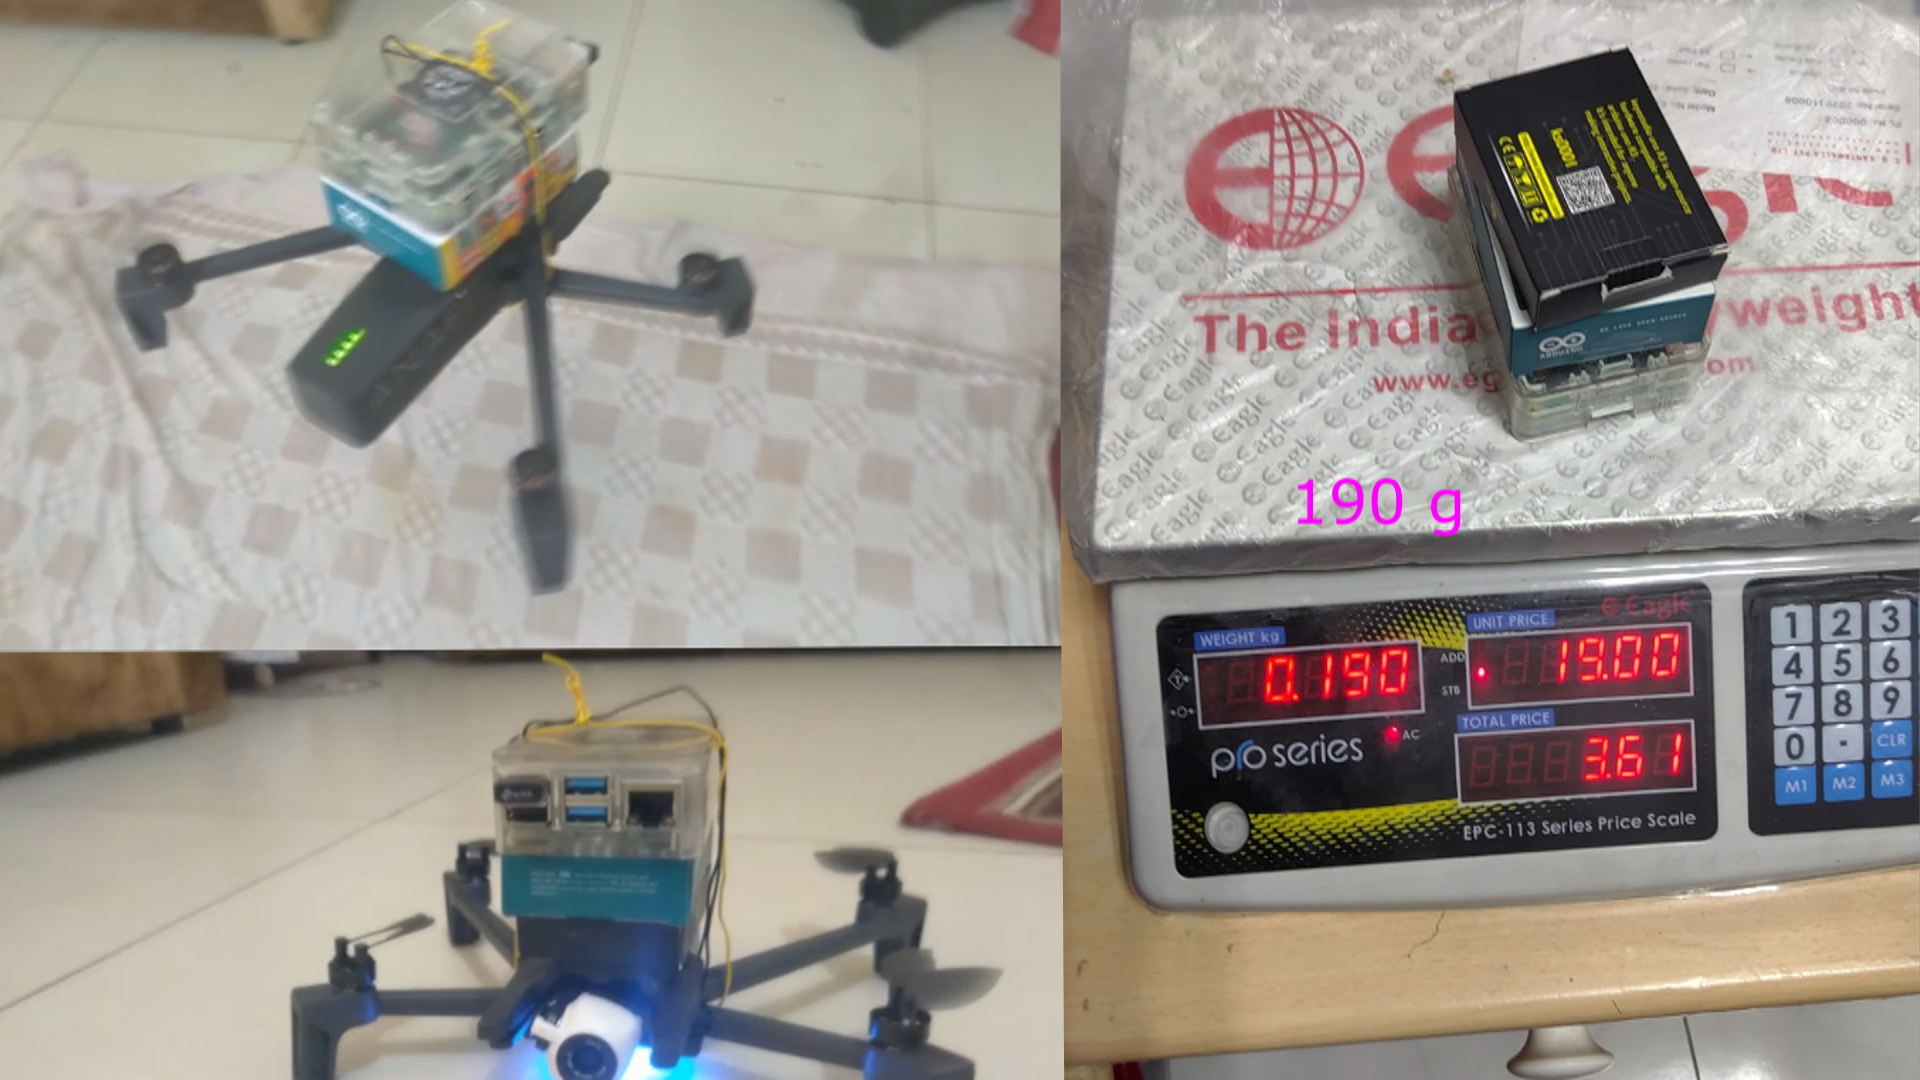
\includegraphics[width=0.6\textwidth]{payload.png}
	\caption{The drone payload}
	\label{fig:payload}
\end{figure} 

For Raspberry Pi power supply it can be connected in 
two different options as shown in \cref{fig:connection}, 
for option A we can use USB-A to power the Raspberry directly without
need to solder any wires,
but there is some internal resistance,
in option B it Power the Raspberry Pi through the \textsc{gpio} 
interface by soldering two wires to the motherboard and 
connect to pin 4 and 6 in the Raspberry Pi board,
this option has small internal resistance compared to option A.
For simplicity, we will choose option A and we will 
follow the instruction of the manufacture by choosing 
the thickest and shortest possible USB cable to reduce 
the cable loss and voltage drops~\cite{makerfocus}. 	 
 
 \begin{figure}[h]
 	\centering
 	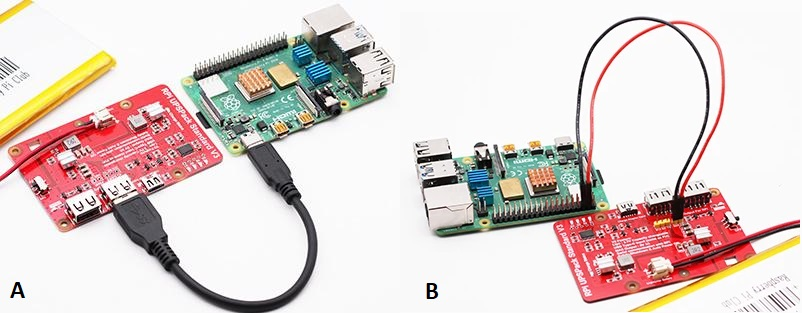
\includegraphics[width=0.6\textwidth]{connection.png}
 	\caption{The Raspberry Pi and power board connection.}
 	\label{fig:connection}
 \end{figure}   

\end{document}
